\documentclass[12pt]{book}

\usepackage[utf8]{inputenc}
\usepackage[russian]{babel}

\usepackage{listings} % staff to show JavaScript code
\usepackage{color} % staff to show JavaScript code
\definecolor{lightgray}{rgb}{.97,.97,.97} % staff to show JavaScript code
\definecolor{darkgray}{rgb}{.4,.4,.4} % staff to show JavaScript code
\definecolor{purple}{rgb}{0.65, 0.12, 0.82} % staff to show JavaScript code

\lstdefinelanguage{JavaScript}{
  keywords={typeof, new, true, false, catch, function, return, null, catch, switch, var, if, in, while, do, else, case, break},
  keywordstyle=\color{blue}\bfseries,
  ndkeywords={class, export, boolean, throw, implements, import, this},
  ndkeywordstyle=\color{darkgray}\bfseries,
  identifierstyle=\color{black},
  sensitive=false,
  comment=[l]{//},
  morecomment=[s]{/*}{*/},
  commentstyle=\color{purple}\ttfamily,
  stringstyle=\color{red}\ttfamily,
  morestring=[b]',
  morestring=[b]"
}

\lstset{
   language=JavaScript,
   backgroundcolor=\color{white},
   extendedchars=true,
   basicstyle=\footnotesize\ttfamily,
   showstringspaces=false,
   showspaces=false,
%   numbers=left,
   numberstyle=\footnotesize,
   numbersep=9pt,
   tabsize=2,
   breaklines=true,
   showtabs=false,
   captionpos=b
}

\begin{document}

%\begin{lstlisting}[caption=My Javascript Example] %example of listining
%Name.prototype = {
%  methodName: function(params){
%    var doubleQuoteString = "some text";
%    var singleQuoteString = 'some more text';
%    // this is a comment
%    if(this.confirmed != null && typeof(this.confirmed) == Boolean && this.confirmed == true){
%      document.createElement('h3');
%      $('#system').append("This looks great");
%      return false;
%    } else {
%      throw new Error;
%    }
%  }
%}
%\end{lstlisting}

\chapter{Все что нужно знать о React}

\chapter{Делаем код чище}

Чтобы использовать JSX без проблем, необходимо понимать как он работает под капотом и почему его удобно использовать для создания интерфейса.

Наша цель - писать чистый и поддерживаемый JSX код, и для этого мы должны знать, как JSX транслируется в JavaScript код и какие предоставляет фичи.

В этом блоке мы разберем:

\begin{itemize}
  \item Что такое JSX и почему мы должны его использовать
  \item Что такое Babel и как он используется в современной разработке
  \item Основные фичи JSX и его отличие от HTML
  \item Лучшие практики при написании кода на JSX
  \item Статическую проверку кода с ESLint 
  \item Основы функционального программирования и его применение в создании React компонент
\end{itemize}


\section{JSX}

**Example of JSX

React предлагает два основных способа описания элементов: использование библиотечных JavaScript функций и использование JSX разметки, похожей на XML. 

На первый взгляд может показаться, что JSX - это странная смесь из HTML и JavaScript. Но на деле, JSX разметка перед попаданием в браузер конвертируется в чистый JavaScript. Этот прием позволяет достаточно лаконично и визуально понятно описывать компоненты.

\subsection{Babel}

Чтобы использовать JSX(а также фичи ES2015) нам необходимо установить Babel. 

Важно понимать, почему мы добавляем Babel в наш процесс разработки. Основная причина в желании использовать фичи языка, которые еще не доступны в браузере. Новые фичи языка часто помогают нам писать код чище и понятнее, но браузер не может их исполнить.

Решение - писать код с JSX и ES2015, а затем транслировать в ES5, который сейчас могут запускать большинство браузеров, используя Babel.

Чтобы использовать Babel, его необходимо установить:

\begin{lstlisting}[language=bash]
	npm install --global babel-cli
\end{lstlisting}

Чтобы не загромождать npm пакетами систему, можно установить babel в конкретный проект и использовать через npm скрипты. Но для учебных целей установим его глобально.

После установки мы можем транслировать любой JavaScript файл:

\begin{lstlisting}[language=bash]
	babel source.js -o output.js
\end{lstlisting}

Одна из сильных сторон Babel - возможность его гибкой конфигурации. Babel всего лишь транслирует один файл в другой, а чтобы были произведены изменения содержимого, нужно сконфигурировать этот процесс.

Для Babel уже создано множество пресетов, в том числе и для JSX и ES2015. Чтобы установить их, необходимо выполнить:

\begin{lstlisting}[language=bash]
npm install --global babel-preset-es2015 babel-preset-react	
\end{lstlisting}

а также добавить в домашнюю директорию (или в папку с проектом) файл .babelrc с содержимым:

\begin{lstlisting}[language=JavaScript]
{
  "presets": [
    "es2015",
    "react" 
  ]
}

\end{lstlisting}

С этого момента мы можем спокойно использовать все фичи ES2015 и JSX, а потом запускать в браузере транслированный Babel'ем код.

\subsection{Hello, World}

Посмотрим на простейший пример создание элемента в React. 

Мы можем создать \textit{div} элемент с помощью метода \textit{createElement} библиотеки React:

\begin{lstlisting}
	React.createElement('div')
\end{lstlisting}

Также мы можем создать его, используя JSX:

\begin{lstlisting}
	<div />
\end{lstlisting}

В данном примере JSX код выглядит как HTML. Но нужно понимать одну важную вещь, оба варианта, написанные выше, эквивалентны. 

На самом деле, если мы транслируем <div /> в JavaScript при помощи babel, то мы получим React.createElement('div'). Это необходимо всегда держать в голове при описании интерфейса на React.

\subsection{DOM элементы и React компоненты}

C JSX мы можем создавать и HTML элементы и React элементы. Разница лишь в том, пишем мы название элемента с заглавной буквы или нет.

Например, в JSX мы можем создать <button /> и <Button /> элементы.

В первом случае результатом трансляции будет:

\begin{lstlisting}
React.createElement('button')
\end{lstlisting}

Во втором случае:

\begin{lstlisting}
React.createElement(Button)
\end{lstlisting}

Разница в том, что в первом случае тип DOM элемента передается как строка, а во втором случае мы передаем название переменной, которая должна быть как минимум определена в области видимости данного кода.

\subsection{Props}

JSX очень удобен, если у DOM или React компонентов есть параметры. В XML в целом гораздо нагляднее передавать параметры элементам:
   
\begin{lstlisting}
<img src="https://facebook.github.io/react/img/logo.svg"
   alt="React.js" />
\end{lstlisting}

Аналогичный код на JavaScript:

\begin{lstlisting}
React.createElement("img", {
     src: "https://facebook.github.io/react/img/logo.svg",
     alt: "React.js"
});
\end{lstlisting}

Читаемость резко падает даже с небольшим количеством параметров.

\subsection{Children}

JSX позволяет определять дочерние элементы, чтобы создавать комплексные древовидные разметки.

Простой пример дочернего элемента - текст внутри тега:

\begin{lstlisting}
<a href="https://facebook.github.io/react/">Click me!</a>
\end{lstlisting}

Этот пример будет транслирован в:

\begin{lstlisting}
React.createElement(
  "a",
  { href: "https://facebook.github.io/react/" },
  "Click me!"
);
\end{lstlisting}
   
Если этот тег будет обернут в другой, например div, то JSX будет выглядеть как:

\begin{lstlisting}
<div>
  <a href="https://facebook.github.io/react/">Click me!</a>
</div>
\end{lstlisting}

JavaScript эквивалентный этому JSX:

\begin{lstlisting}
React.createElement(
  "div",
  null,
  React.createElement(
    "a",
    { href: "https://facebook.github.io/react/" },
    "Click me!"
  ) 
);
\end{lstlisting}

Достаточно очевидно, что чем сложнее разметка, тем больше JSX улучшает читаемость кода. Однако не следует забывать, что каждому JSX коду соответствует однозначно определенный код на JavaScript.

Так как JSX всего лишь удобный синтаксис для JavaScript, вполне логично, что в нем можно использовать JavaScript выражения. 

Для того, чтобы сделать это, выражение должно быть обернуто в фигурные скобки:

\begin{lstlisting}
<div>
  Hello, {variable}.
  I'm a {function()}.
</div>	
\end{lstlisting}


Или например в параметрах элемента:

\begin{lstlisting}
<a href={this.makeHref()}>Click me!</a>
\end{lstlisting}

\subsection{Differences with HTML}

Мы посмотрели, чем похожи JSX и HTML. Теперь посмотрим в чем они отличаются и в чем причины этих различий.

\subsubsection{Аттрибуты}

Мы должны помнить, что JSX не стандарт языка, и транслируется в JavaScript. Из-за этого некоторые атрибуты не доступны для использования.

Например, вместо атрибута class мы вынуждены использовать className, а вместо for использовать htmlFor:

\begin{lstlisting}
<label className="awesome-label" htmlFor="name" />
\end{lstlisting}

Причина этого в том, что слова class и for зарезервированы в языке JavaScript.

\subsubsection{Стили}

Стили - пример значительных различий между HTML и JSX. Подробнее мы посмотрим на них в одной из следующих глав. 

Сейчас отметим, что через JSX в атрибуте style не поддерживается CSS строка. Вместо нее React ожидает JavaScript объект, в котором имена стилей переданы в camelCase:

\begin{lstlisting}
<div style={{ backgroundColor: 'red' }} />
\end{lstlisting}

\subsubsection{Root}

Стоит отметить важное отличие JSX от HTML, которое заключается в том, что нельзя создать несколько элементов на одном уровне без оборачивания другим элементом:

\begin{lstlisting}
<div />
<div />
\end{lstlisting}

Этот пример вызовет следующую ошибку:

Adjacent JSX elements must be wrapped in an enclosing tag

Проблема решается добавлением общего элемента:

\begin{lstlisting}
<div> 
  <div />
  <div />
</div>
\end{lstlisting}
   
Это происходит из-за того, что каждый элемент в JSX транслируется в React.createElement в JavaScript, а в JavaScript нельзя вернуть из функции результат работы двух последовательных вызовов какой-либо функции.

Сейчас React предоставляет возможность использовать пустой тег, чтобы отрисовывать несколько элементов на одном уровне:

\begin{lstlisting}
render() {
  return (
    <>
      <ChildA />
      <ChildB />
      <ChildC />
    </>
  );
}
\end{lstlisting}
  
\subsubsection{Spaces}   

Есть еще одна мелочь, которая может вводить в ступор новичков, которая заключается в различной обработке пробельных символов в HTML и JSX.

Например, рассмотрим следующий пример кода, который корректен и в HTML и в JSX:

\begin{lstlisting}
<div>
  <span>foo</span>
  bar
  <span>baz</span>
</div>
\end{lstlisting}

Если открыть этот кусочек напрямую в браузере как HTML файл, то мы увидим foo bar baz. А если мы добавим его в JSX, то после отрисовки будет foobarbaz.

Это происходит из-за того, что JSX воспримет три строки внутри div, как три дочерние элементы и проигнорирует пробельные символы, а после отрисовке все три дочерних элемента будут отрисованы один за другим.

Основной способ исправить это, добавить еще дочерние элементы, которые будут также являться дочерними элементами:

\begin{lstlisting}
<div>
  <span>foo</span>
  {' '}
  bar
  {' '}
  <span>baz</span>
</div>
\end{lstlisting}

Таким образом мы добавляем пустые строки, которые являются JavaScript выражениями, чтобы заставить компилятор добавить новые дочерние элементы.

\subsubsection{Boolean атрибуты}

Также есть небольшое отличие в использовании boolean атрибутов в JSX. Если передать какой-либо атрибут без значения, то JSX поймет, что это boolean атрибут со значением true:

\begin{lstlisting}
<button disabled />
\end{lstlisting}

\begin{lstlisting}
React.createElement("button", { disabled: true });
\end{lstlisting}
   
Но в отличие от HTML, чтобы передать атрибут со значением false, необходимо сделать это в явном виде. Если не передать атрибут совсем, то он не попадет в передаваемый объект с атрибутами, и при дальнейшей попытке использования может быть получен undefined вместо false, что приводит к потенциальным ошибкам:

\begin{lstlisting}
<button disabled={false} />
\end{lstlisting}

\begin{lstlisting}
React.createElement("button", { disabled: false });
\end{lstlisting}
   
Эта особенность может вводить в заблуждение, так как в HTML принято отсутствие атрибута считать как false значение для этого атрибута. В React следует всегда явным образом указывать значение boolean атрибутов.

\subsection{Spread атрибут}

Важная особенность JSX - \textbf{spread атрибуты}, которая приходит из стандарта ECMASript (https://github.com/sebmarkbage/ecmascript-re st-spread) и очень удобно в случае, когда нам нужно передать все атрибуты JavaScript объекта в параметры элементу.

Распространенная практика - избежать передачи объекта дочерним элементам по ссылке во избежании ошибок, связанных с изменяемостью таких объектов.

В качестве примера можем посмотреть на код:

\begin{lstlisting}
const foo = { id: 'bar' }
return <div {...foo} />
\end{lstlisting}
   
который будет транслирован в следующий JSX код:

\begin{lstlisting}
var foo = { id: 'bar' };
return React.createElement('div', foo);
\end{lstlisting}
   
\subsection{Шабоны JavaScript}

Мы начали с предположения, что одно из преимуществ использования шаблонов внутри наших компонент вместо использования сторонних библиотек шаблонов(прим.пер. видимо имеются ввиду библиотеки-шаблонизаторы как handlebars) в использовании всей мощи языка JavaScript внутри шаблонов.

Spread оператор один из примеров использования JavaScript внутри JSX. Но в целом любое JavaScript выражение может быть использовано как атрибут элемента, для этого достаточно обернуть его в фигурные скобки:

\begin{lstlisting}
<button disabled={errors.length} />
\end{lstlisting}

\subsection{Основные паттерны}

Мы разобрались с тем, как работает JSX. Теперь мы можем можем подумать детальнее, как использовать JSX, следуя полезным соглашениям и практикам.

\subsubsection{Многострочный JSX код}

Начнем с простого примера. Одна из причин использовать JSX вместо React.createElement - наглядность XML-like синтаксиса, а также потому что такая структура из отрывающих и закрывающих тегов идеально подходит для описания древовидных структур.

Например, если у нас есть JSX код с множеством вложенных элементов, мы должны предпочитать многострочную запись JSX кода однострочной:

\begin{lstlisting}
<div>
  <Header />
  <div>
    <Main content={...} />
  </div>
</div>
\end{lstlisting}

Такой вариант гораздо предпочтительнее, чем:

\begin{lstlisting}
<div><Header /><div><Main content={...} /></div></div>
\end{lstlisting}

Однако, если дочерний элемент - не React элемент, а текст или переменная, то разумнее будет записать весь тег в одной строке:

\begin{lstlisting}
<div>
  <Alert>{message}</Alert>
  <Button>Close</Button>
</div>
\end{lstlisting}

Также рекомендуется оборачивать все JSX блоки в круглые скобки. Это необходимо делать, чтобы не было проблем с автоматической вставкой точки с запятой. Проблемы могут возникнуть, если например, немного не аккуратно вернуть. JSX разметку из функции.

Следующий пример отработает корректно, так как return и div находятся на одной линии:

\begin{lstlisting}
return <div />
\end{lstlisting}

Но следующий уже отработает непредвиденным образом:

\begin{lstlisting}
return
     <div />
\end{lstlisting}
     
Проблема кроется в том, что во втором случае JSX код будет транслирован в следующий JavaScript код:

\begin{lstlisting}
return;
React.createElement("div", null);
\end{lstlisting}
   
Чтобы избежать таких проблем, рекомендуется всегда оборачивать многострочные JSX элементы в круглые скобки:

\begin{lstlisting}
return (
  <div />
)
\end{lstlisting}

\subsubsection{Multi-properties}

Небольшой проблемой является также множество атрибутов у элемента. Если записывать атрибуты в одну строку, то она может начать занимать много места в ширину и быть неудобной для чтения. 

Поэтому стоит стараться писать каждый атрибут в новой строке, а закрывающий тег выравнивать с открывающим (прим.пер. также хороший вариант - оставлять закрывающий тег на одной строке с последним атрибутом):

\begin{lstlisting}
<button
  foo="bar"
  veryLongPropertyName="baz"
  onSomething={this.handleSomething}
/>
\end{lstlisting}

\subsubsection{Условные операторы}

Все гораздо интереснее с использование \textbf{условий} в JSX, например, если нужно отрисовать какой-то компонент только при каком-то условии. С одной стороны возможность использовать JavaScript внутри JSX - большой плюс, но с другой стороны у нас появляется множество вариантов использования условий и нужно знать об их плюсах и минусах.

Предположим, что нам нужно отрисовать кнопку logout только для авторизованного пользователя. Простой вариант решения этой проблемы может выглядеть следующим образом:

\begin{lstlisting}
let button
if (isLoggedIn) {
  button = <LogoutButton />
}
return <div>{button}</div>
\end{lstlisting}
   
Это работает, но этот вариант плохо читается, если у нас есть множество условий и множество элементов.

Также мы можем использовать ленивую проверку логических выражений в JavaScript:

\begin{lstlisting}
<div>
  {isLoggedIn && <LoginButton />}
</div>
\end{lstlisting}

Это работает, так как в случае false в isLoggedIn JavaScript не будет проверять остальное выражение, а если true, тогда вызовется createElement для LoginButton и результат ее работы вернется как результат всего выражения.

Если мы хотим, чтобы в условии была также альтернативная ветка, например чтобы показать разные кнопки для авторизованного и неавторизованного пользователей, то мы может использовать if...else в JavaScript:

\begin{lstlisting}
let button
if (isLoggedIn) {
  button = <LogoutButton />
} else {
  button = <LoginButton />
}
return <div>{button}</div>
\end{lstlisting}
   
Помимо этого мы можем использовать тернарный оператор, чтобы сделать код компактнее:

\begin{lstlisting}
<div>
  {isLoggedIn ? <LogoutButton /> : <LoginButton />}
</div>
\end{lstlisting}

Можно найти множество примеров использования тернарных операторов в известных репозиториях, например в Redux(https://github.com/reactjs/redux/blob/master/examples/real-world/src/components/List.js\#L25), где он используется для показа разного текста в зависимости от того, грузятся ли данные по сети:

\begin{lstlisting}
<button [...]>
  {isFetching ? 'Loading...' : 'Load More'}
</button>
\end{lstlisting}

Посмотрим, что произойдет, если логическое выражение будет становиться сложнее и в нем будут задействованы разные переменные и логические операции:

\begin{lstlisting}
<div>
  {dataIsReady && (isAdmin || userHasPermissions) && 
    <SecretData />
}
</div>
\end{lstlisting}

Это решение все еще может быть неплохим, но читаемость его начинает падать. Для решения этой проблемы можно создать вспомогательную функцию внутри компонента и использовать ее название для пояснения логики, сокрытой в теле:

\begin{lstlisting}
canShowSecretData() {
  const { dataIsReady, isAdmin, userHasPermissions } = this.props
  return dataIsReady && (isAdmin || userHasPermissions)
}
<div>
  {this.canShowSecretData() && <SecretData />}
</div>
\end{lstlisting}

Код стал более читаемым, и даже если вернуться к нему через полгода, достаточно будет прочесть название функции и опустить чтение логики внутри.

Если вы не любите использовать функцию, то ее можно заменить геттеро, который сделат код более элегантным (прим.пер. а может быть и нет...):

\begin{lstlisting}
get canShowSecretData() {
  const { dataIsReady, isAdmin, userHasPermissions } = this.props
  return dataIsReady && (isAdmin || userHasPermissions)
}
<div>
  {this.canShowSecretData && <SecretData />}
</div>
\end{lstlisting}

То же самое относится к вычисляемым значениям. Например, если у нас есть два значения, валюта и стоимость, и нам нужно объединить их в одну строку, то мы можем вынести эту операцию в отдельный метод.

\begin{lstlisting}
getPrice() {
  return `${this.props.currency}${this.props.value}`
}
<div>{this.getPrice()}</div>
\end{lstlisting}

Это также удобнее тестировать, если внутри этого метода есть дополнительная логика.

То же самое можно сделать с помощью геттеров аналогично предыдущим примерам:

\begin{lstlisting}
get price() {
  return `${this.props.currency}${this.props.value}`
}
<div>{this.price}</div>
\end{lstlisting}

Есть еще множество решений проблемы ветвления внутри React компонент, которое требует использования сторонних библиотек. В общем случае стоит аккуратно вносить новые зависимости в проект, так как они могут увеличить размер бандла, принести проблему на смене версий и увеличить порог входа в проект, но на что не пойдешь ради увеличения читаемости кода (прим.пер. используемые тут библиотеки довольно просты и имеет смысл реализовать их самостоятельно в учебных целях).

Первый вариант - использовать библиотеку render-if, которую можно установить командой:
\begin{lstlisting}[language=bash]
npm install --save render-if
\end{lstlisting}

Мы можем легко использовать ее в проекте по аналогии с примером ниже:

\begin{lstlisting}
const { dataIsReady, isAdmin, userHasPermissions } = this.props
const canShowSecretData = renderIf(
  dataIsReady && (isAdmin || userHasPermissions)
)
<div>
  {canShowSecretData(<SecretData />)}
</div>
\end{lstlisting}


Мы оборачиваем наше условии внутри renderIf функции.

Результатом вызова функции renderIf является функция, которая принимает аргументом React элемент, который она вернет при вызове в случае истинности условия.

Самое главное, что мы не должны забывать в данном контексте, это то, что компоненты должны оставаться простыми и глупыми настолько насколько это возможно. Иначе в этих компонентах будет сложно разбираться, править баги и расширять.

Чтобы сделать компонент чище, мы можем вынести из него логику в Компонент более высокого порядка (Higher-Order Component, HOC) с библиотекой react-only-if. Компоненты выского порядка мы рассмотрем далее в Главе 4, сейчас для нас важно только то, что HOC это функция, которая принимает аргументом компонент, расширяет его или изменяет его поведения и возвращает при вызове.

Данная библиотека устанавливается командой:

\begin{lstlisting}[language=bash]
npm install --save react-only-if
\end{lstlisting}

После установки мы можем использовать ее внутри нашего приложения следующим образом:

\begin{lstlisting}
const SecretDataOnlyIf = onlyIf(
  ({ dataIsReady, isAdmin, userHasPermissions }) => {
    return dataIsReady && (isAdmin || userHasPermissions)
  }
)(SecretData)
<div>
  <SecretDataOnlyIf
    dataIsReady={...}
    isAdmin={...}
    userHasPermissions={...}
  /> 
</div>
\end{lstlisting}

Как можно заметить, в этом случае внутри исходного компонента нет логики совсем, что повышает его тестируемость.

Мы передаем условие как параметр в функцию onlyIf, которая меняет поведение нашего компонента таким образом, чтобы оно отображалось только в случае истинности логического выражения.

\subsubsection{Циклы}

Отображения списков элементов - очень распространенная операция. И в данном случае JavaScript показывает себя с хорошей стороны.

Если мы поместим внутрь JSX массив с React элементами, то все они будут отрисованы на одном уровне вложенности. В целом для нас не важно, как будет получен этот массив, главное, чтобы как и любое другое выражение, было помещено в фигурные скобки.

Самым распространенным способом создать массив элементов является использование операций над множествами объектов языка JavaScript:

\begin{lstlisting}
<ul>
  {users.map(user =><li>{user.name}</li>)}
</ul>
\end{lstlisting}

Этот пример прост, но показывает большую гибкость использования JSX и JavaScript для генерации HTML.

\subsubsection{Control statements}

Условные операторы и циклы часто используются для описания верстки и, возможно, вам может показаться, что вносить в JSX блоки JavaScript кода для таких базовых операция - не лучшая практика. Но JSX был разработан лишь как инструмент генерации элементов, оставляя работы с логикой программы на JavaScript.

В общем и целом не стоит держать большой объем логики внутри компонент, но тем не менее время от времени нам нужно скрывать или показывать элементы в зависимости от состояния или итерировать коллекции объектов для отображения списков. 

Если вы чувствуете, что JSX должен также позволять использовать условия и циклы, и это сделает код более читаемым, то вы можете попробовать библиотеку: jsx-control-statements.

Эта библиотека не приносит никакого нового функционала в JSX и являешься лишь синтаксическим сахаром, который компилируется в JavaScript.

Прежде всего нам нужно добавить ее в проет:

\begin{lstlisting}[language=bash]
npm install --save jsx-control-statements
\end{lstlisting}

Также его необходимо добавить в .babelrc, чтобы babel знал, что у нас появились новые правила компиляции:

\begin{lstlisting}
"plugins": ["jsx-control-statements"]
\end{lstlisting}

С этого момента мы можем использовать новый синтакс и babel будет транслировать его вместе со стандартным JSX.

Условный оператор, написанный с использование этого плагина, будет выглядеть следующим образом:

\begin{lstlisting}
<If condition={this.canShowSecretData}>
  <SecretData />
</If>
\end{lstlisting}

Этот код будет транслирован в обычный тернарный оператор в JavaScript:

\begin{lstlisting}
{canShowSecretData ? <SecretData /> : null}
\end{lstlisting}

Для ситуации, когда нам нужно иметь возможность выбрать элемент из нескольких в зависимости от различных условий, в данной библиотеке есть компонент Choose:

\begin{lstlisting}
<Choose>
  <When condition={...}>
    <span>if</span>
  </When>
  <When condition={...}>
    <span>else if</span>
  </When>
  <Otherwise>
    <span>else</span>
  </Otherwise>
</Choose>
\end{lstlisting}

Не стоит забывать, что компоненты Choose, When и Otherwise не являются React компонентами в привычном для нас понимании, это всего лишь синтаксис, который будет скомпилирован в большой набор тернарных операторов.

Также есть специальный компонент For (который также будет скомпилирован в JavaScript код) для работы с коллекциями объектов:

\begin{lstlisting}
<ul>
  <For each="user" of={this.props.users}>
    <li>{user.name}</li>
  </For>
</ul>
\end{lstlisting}

Тут тоже никакой магии, после компиляции этот блок превратится в вызов метода map.

Если вы используете какой-либо линтер, то он может ругаться в последнем случае, так как переменная user по сути не определена. Это происходит из-за того, что объявление этой переменной будет сгенерировано после компиляции.

Если вы используете eslint, то для исключения данной ошибки проверки кода можно использовать библиотеку eslint- plugin-jsx-control-statements.

Если у вас еще нет опыта использования линтеров, то не беспокойтесь, они будут разобраны чуть позже. 

\subsubsection{Sub-rendering}

В общем случае стоит стараться делать компоненты маленькими и простыми насколько это возможно, но тем не менее компоненты могут начать разбухать, особенно если разработка идет итеративно и функционал наращивается понемногу на каждой итерации.

Что мы можем сделать, если наши методы отображения компонент становятся слишком большими. Один из вариантов - разделить большой метод render на небольшие функции внутри одного компонента:

\begin{lstlisting}
renderUserMenu() {
    // JSX for user menu
}
renderAdminMenu() {
    // JSX for admin menu
}
render() {
  return (
    <div>
      <h1>Welcome back!</h1>
      {this.userExists && this.renderUserMenu()}
      {this.userIsAdmin && this.renderAdminMenu()}
    </div> 
  )
}
\end{lstlisting}

Это далеко не идеальное решение, но на практике, если нет возможности разделить компонент на более мелкие, это позволяет сохранять метод render чище.

Теперь мы должны начать чувствовать себя посвободнее в использовании JSX. Можно перейти к вопросу, как следовать единому стилю кода внутри всего проекта.

\section{ESLint}

Мы всегда пытаемся писать лучший код, на который способны, но все равно время от времени делаем ошибки и тратим часы на их поиск и исправление.

К счастью для нас, есть инструменты, которые позволяют искать ошибки еще на стадии написания кода. Такие инструменты не скажут, делает ли код то, что должен, но как минимум помогут избежать синтаксических ошибок.

Если вы пришли из мира языков со статической типизацией, таких как C\#, то вы привыкли, что множество синтаксических ошибок можно обнаружить в IDE во время написания кода.

Дуглас Крокфорд (Douglas Crockford) сделал линтинг (статическую проверку кода) популярным в мире JavaScript с инструментом JSLint(первый релиз в 2002). Дальше этот инструмент перерос в JSHint, а затем в ESLint, став основным инструментом статической проверки кода в JavaScript мире в целом и в React разработке в частности.

\textbf{ESLint} - инструмент с открытым исходным кодом, вышедший в 2013 году и быстро набравший популярность за счет гибкости в настройке и расширении.

В мире JavaScript, где постоянно меняются библиотеки и подходы, возможность гибкой конфигурации стала одной из главных причин быстрого распространения ESLint. 

Помимо этого сейчас мы транслируем код с помощью babel и используем новые возможности языка и сторонние расширения, такие как JSX. Плюс ESLint в том, что он позволяет дописывать расширения для проверки любого нового синтаксиса.

Помимо этого, так как ESLint позволяет создавать правила для проверки синтаксиса, у нас появляется возможность определить единый стиль кода внутри больших команд.


\subsection{Установка}

Прежде всего нам нужно установить ESLint:

\begin{lstlisting}
npm install --global eslint
\end{lstlisting}

После этого мы можем запустить его следующей командой:

\begin{lstlisting}
eslint source.js
\end{lstlisting}

На выходе мы получим информацию об ошибках внутри файла с кодом.

Но при первом запуске мы не должны увидеть никаких ошибок, потому ESLint не содержит никаких правил проверки по умолчанию.

\subsection{Настройка}

Для настройки ESLint используется файл $.eslintrc$ в домашней директории проета или пользователя.

Начнем с простого и запретим использовать символ точки с запятой. Для этого добавим в .eslintrc следующий JSON:

\begin{lstlisting}
{
  "rules": {
    "semi": [2, "never"]
  } 
}
\end{lstlisting}

Эта запись определенно требует некоторых пояснений: $"semi"$ - название правила(rule), а $[2, "never"]$ - его значение. 

В ESLint каждому правилу можно задать один из 3 уровней строгости:

\begin{itemize}
  \item \textbf{off (0): Правило выключено}
  \item \textbf{warn (1): Правило предупреждения}
  \item \textbf{error (2): Правило ошибки}
\end{itemize}

Таким образом, указав в нашем примере значение 2, мы говорим, что ESLint, при срабатывании этого правила, должен ругаться о наличии ошибки в коде.

Второй параметр ($"never"$) говорит о том, что точка с запятой никогда не должна использоваться внутри проекта.

ESLint и его плагины хорошо документированы и можно всегда посмотреть, как именно работают правила, и что значат их аргументы.

Теперь создадим файл index.js со следующим содержимым:

\begin{lstlisting}
var foo = 'bar';
\end{lstlisting}

(Мы используем $var$ так как ESLint еще не знает о том, что мы собираемся использовать ES2015).

Если мы запустим $eslint index.js$, то получим следующее сообщение:

$$\textbf{Extra semicolon (semi)}$$

Заработало, теперь мы можем добавлять правила и следовать (или не следовать) им внутри проекта.

Мы можем добавлять все правила вручную или включить рекомендованный набор правил одной строкой в .eslintrc:

\begin{lstlisting}
{
  "extends": "eslint:recommended"
}
\end{lstlisting}

После этого каждое отдельное правило может быть изменено по необходимости вручную.

После применения рекомендованных правил мы должны перестать получать ошибку о наличии точки с запятой (т.к. это правило не входит в рекомендованные), но должны получить ошибку, что переменная $foo$ объявлена, но никогда не используется.

Правило $no-unused-vars$ очень полезно для сохранения чистоты кодовой базы.

Вспомним, что мы хотим писать код на ES2015, но если мы изменим исходный код на следующий:

\begin{lstlisting}
const foo = 'bar'
\end{lstlisting}

То получим следующую ошибку:

$$
\textbf{Parsing error: The keyword 'const' is reserved}
$$

Для того, чтобы включить поддержку ES2015, мы должны добавить информацию об этом в .eslintrc:

\begin{lstlisting}
"parserOptions": {
  "ecmaVersion": 6,
}
\end{lstlisting}

Также для нас будет полезно указать, что мы используем JSX:

\begin{lstlisting}
"parserOptions": {
  "ecmaVersion": 6,
  "ecmaFeatures": {
    "jsx": true 
  }
},
\end{lstlisting}

Если вы уже писали приложения на React, но не использовали линтер, то хорошим упражнением будет добавить ESLint в уже существующий проект и исправить все ошибки, которые будут найдены.

Использование ESLint из консоли конечно позволяет нам проверять код, но еще одним плюсом этого инструмента является то, что он поддерживается большинством современных редакторов и IDE (SublimeText, Atom и множество других).

Очень часто есть сильный соблазн просто проигнорировать все, что говорит нам ESLint и залить код в общий репозиторий. Чтобы избежать этого, имеет смысл добавить линтер как один из шагов в процесс сборки приложения, в этом случае код с ошибками просто не попадет в продакшн.

Еще вариант, добавить линтер на этап создания пулл реквета. В этом случае код с ошибками не попадет даже на ревью кода.

\subsection{React плагин}

Как было сказано раньше, одна из сильнейших сторон ESLint - его расширяемость плагинами. Самый важный плагин для нас eslint-plugin-react.

В целом ESLint может работать с JSX без дополнительных плагинов. Но мы хотим больше, например хранить наши компоненты в одном определенном стиле.

Прежде всего нам нужно установить плагин:

\begin{lstlisting}
npm install --global eslint-plugin-react
\end{lstlisting}
   
После этого мы можем добавить его в наш файл с настройками:

\begin{lstlisting}
"plugins": [
  "react"
]
\end{lstlisting}

По аналогии с самим ESLint мы можем добавить набор рекомендованных настроек для react плагина:

\begin{lstlisting}
"extends": [
  "eslint:recommended",
  "plugin:react/recommended"
],
\end{lstlisting}

С этого момента, если что-то будет не так с нашими компонентами, например мы попробуем передать один и тот же параметр дважды, ESLint будет предупреждать об ошибке:

\begin{lstlisting}
<Foo bar bar />
\end{lstlisting}

И соответствующее сообщение об ошибке:

$$
\textbf{No duplicate props allowed (react/jsx-no-duplicate-props)}
$$

Есть множество правил, которые мы можем использовать в нашем проекте. Давайте посмотрим, как некоторые из них могут улучшить нашу жизнь.

Одна из проблем, которую может помочь решить для нас ESLint, - это одинаковый размер отступов в JSX верстке. Это поможет нам сохранить единый стиль внутри всего приложения и не держать постоянно в голове точный размер отступов.

Для того, чтобы включить эту проверку, достаточно добавить следующее правило:

\begin{lstlisting}
"rules": {
  "react/jsx-indent": [2, 2]
}
\end{lstlisting}

Первая $2$ означает, что ESLint будет говорить об ошибке, если сработает это правило, вторая $2$ говорит от том, что размер отступа для каждого компонента должен быть из двух пробелов. Также можно сказать, что отступов не должно быть вовсе, заменив вторую $2$ на $0$.

Создайте файл с содержимым вида:

\begin{lstlisting}
<div>
<div />
</div>
\end{lstlisting}

И вы получите ошибку:

$$
\textbf{Expected indentation of 2 space characters but found 0 (react/jsx-indent)}
$$

Аналогичным образом мы можем заставить всех использовать одинаковый отступ для всех параметров элементов:

\begin{lstlisting}
"react/jsx-indent-props": [2, 2]
\end{lstlisting}

Также часто возникают вопросы, на которые у каждого разработчика может найтись свое мнение отличное от других. Например, какой максимальной длины должны быть строки кода? Или когда считать, что у элемента слишком много параметров? С ESLint и правилом jsx-max-props-per-line можно выбрать единое значение для всех, чтобы не возвращаться к этому вопросу на каждом ревью кода.

React плагин для ESLint позволяет проверять не только JSX, но и сами компоненты. 

Например, мы можем договориться определять PropTypes в алфавитном порядке. Есть правило, чтобы проверить, что используются только объявленные в PropTypes параметры. Или правило для проверки того, что все компоненты без состояния объявлены в функциональном стиле. А также множество других правил.

\subsection{Airbnb configuration}

Мы уже посмотрели, как ESLint помогает искать ошибки и следовать единому стилю кода. Также мы увидели, насколько ESLint открыт для настройки и расширения.

Можно сделать шаг дальше.

Через атрибут extends в файле настроек ESLint можно подключить конфигурации сторонних организаций, а затем уже добавлять свои правила поверх них.

Одна из самых известных конфигураций для ESLint в мире React была создана в стенах компании Airbnb. Разработчики этой компании создали набор правил, чтобы следовать единому стилю кода среди всех разработчиков, и каждый желающий может подключить этот набор правил в свой проект.

Для того, чтобы сделать это необходимо добавить несколько зависимостей:

\begin{lstlisting}
npm install --global eslint-config-airbnbeslint@^2.9.0 eslint-plugin-jsx-a11y@^1.2.0 eslint-plugin-import@^1.7.0 eslint-plugin-react@^5.0.1
\end{lstlisting}

А затем добавить новые настройки в .eslintrc:

\begin{lstlisting}
{
  "extends": "airbnb"
}
\end{lstlisting}

Это один из самых простых и распространенных способов начать работать с ESLint.


\section{Основы функционального программирования}

Кроме исправления JSX и использования линтера есть еще один способ сделать код чище: следовать \textbf{Функциональному (Functional Programming, FP)} стилю.

Функциональное программирование - парадигма декларативного программирования, сосредоточенная на минимизации побочных эффектов (side effects) и сохранении данных неизменяемыми (immutable).

Следующая часть не ставит своей целью полностью раскрыть обширную тему функционального программирования, но мы можем посмотреть на некоторые концепции, которые часто используются в React. 

\subsection{Объект первого класса}

В JavaScript функции являются \textit{объектами первого класса (first-class objects)}, т.е. они могут быть присвоены переменным как значение и переданы как аргументы другим функциям.

Это позволяет нам ввести концепцию \textbf{Функций высшего порядка (Higher-order Functions, HoF)}. Такой функцией мы будем назвать функцию, которая принимает аргументом функцию (и возможно другие аргументы) и возвращает новую функцию. Возвращаемая функция чаще всего расширяет функционал изначальной функции.

Посмотрим на простой пример, функцию сложения двух чисел, которую мы обернем функцией, логирующей все аргументы функции и вызывающей изначальную функцию сложения:

\begin{lstlisting}
const add = (x, y) => x + y

const log = func => (...args) => {
  console.log(...args)
  return func(...args)
}
const logAdd = log(add)
\end{lstlisting}

Функции высшего порядка часто используется в React разработке. Один из самых распространенных паттернов использования этого приема - \textbf{Компоненты высшего порядка (Higher-order Components, HoC)}. Подробнее на компоненты высшего порядка мы посмотрим в Главе 4.

\subsection{Purity}

Важный аспект функционального программирования - чистые функции. С ними вы будете встречаться очень часто, особенно в таких библиотеках как Redux.

Главное отличие чистой функции - отсутствие побочных эффектов.

К примеру, если функция меняет состояние приложения, меняет значение переменных во внешней области видимости переменных или меняет значение переменных переданных по ссылке, то функция не является чистой.

Чистые функции значительно проще тестировать так как при вызовах с одинаковыми аргументами функция возвращает одинаковый результат.

Простой пример чистой функции - функция сложения:

\begin{lstlisting}
const add = (x, y) => x + y 
\end{lstlisting}

Она может быть запущена множество раз с одними и те ме же аргументами, но в каждый раз она вернет одинаковый результат. 

В следующем примере функция перестает быть чистой:

\begin{lstlisting}
let x = 0
const add = y => (x = x + y)
\end{lstlisting}

Если мы вызовем $add(1)$ дважды, то сначала мы получим $1$, а затем $2$. Причина в том, что работа функции зависит от переменной во внешней области видимости, которая еще и редактируется внутри этой функции.

\subsection{Immutability}

Мы разобрались с чистыми функциями, которые не изменяют состояние приложения, но что если в функцию приходит сложный объект, в котором мы хотим что-либо изменить? 

FP говорит нам о том, что в этом случае следует создать новый объект с измененным значением и вернуть его, не трогая исходный объект.

Рассмотрим пример:

\begin{lstlisting}
const add3 = arr => arr.push(3)
const myArr = [1, 2]
add3(myArr) // [1, 2, 3]
add3(myArr) // [1, 2, 3, 3]
\end{lstlisting}

Эта функция изменяет состояние исходного массива, что противоречит парадигме неизменяемости. Если вызвать эту функцию несколько раз с одним и тем же исходными массивом, то мы будем получать разные значения на выходе.

Мы можем исправить эту функцию, чтобы она стала immutable с помощью метода concat, который возвращает новый массив, оставляя исходный без изменений:

\begin{lstlisting}
const add3 = arr => arr.concat(3)
const myArr = [1, 2]
const result1 = add3(myArr) // [1, 2, 3]
const result2 = add3(myArr) // [1, 2, 3]
\end{lstlisting}

Или используя спред оператор:

\begin{lstlisting}
const add3 = arr => [...arr, 3]
\end{lstlisting}

Сколько бы мы ни вызывали этот метод, исходный массив остается нетронутым. 

\subsection{Каррирование}

\textbf{Каррирование (Curring)} - еще одна распространенная техника функционального программирования, которая заключается в конвертации функции от многих переменных в функцию одной переменной, которая возвращает другую функцию.

Посмотрим на примере функции $add$ как это работает на практике. Вместо исходной функции от двух аргументов:

\begin{lstlisting}
const add = (x, y) => x + y
\end{lstlisting}

Мы можем определить каррированную функцию:

\begin{lstlisting}
const add = x => y => x + y
\end{lstlisting}

Такую функцию мы можем использовать следующим образом:

\begin{lstlisting}
const add1 = add(1)
add1(2) // 3
add1(3) // 4
\end{lstlisting}

Таким способом мы можем заключить первый аргумент внутри переменной $add1$ и использовать ее множество раз без явной передачи.

\subsection{Композиция}

Композиция (Composition) - еще один прием, который позволяет сохранять функции небольшими и тестируемыми.

Рассмотрим следующий пример:

\begin{lstlisting}
const add = (x, y) => x + y
const square = x => x * x
\end{lstlisting}

Эти функции могут быть скомбинированы вместе, чтобы создать новую функцию, которая складывает два числа и возвращает их квадрат:

\begin{lstlisting}
const addAndSquare = (x, y) => square(add(x, y))
\end{lstlisting}

Следуя этому простому приему можно сохранять функции небольшими и читаемыми, а также упростить их тестирование.



\subsection{FP и пользовательские интерфейсы}

Последний шаг - понять, как функциональное программирование помогает нам строить пользовательский интерфейс. 

Мы можем думать о UI как о функции, которая принимает аргументом состояние приложения, а возвращает интерфейс приложения:

$$
UI = f(state)
$$

Мы хотим ожидать, что эта функция будет чистой, т.е. для одного и того же состояния приложения она будет возвращать всегда одинаковое представление для пользователя.

В React мы будем будем рассматривать компоненты как функции и комбинировать из этих функций пользовательский интерфейс.

Есть много схожего между функциональным программирование и созданием пользовательского интерфейса с React. И чем больше мы будем смотреть на разработку с React как на функциональное программирование, тем лучше будет наш код.

\section{Заключение}

В этой главе мы детально разобрали строение JSX и как с помощью него создавать компоненты. 

Также мы разобрались со статической проверкой кода средствами ESLint и его плагинов. Это позволит нам быстрее находить потенциальные проблемы в коде.

И в конце мы рассмотрели базовые концепции функционального программирования, которые часто встречаются в React. 

Используя все выше сказанное, можно сделать код значительно чище и более тестируемым. Настало время сделать еще один шаг вперед и разобраться, как сделать действительно переиспользуемые компоненты.


\chapter{Создаем реально переиспользуемые компоненты}

Для того чтобы создавать действительно переиспользуемые компоненты мы должны разобраться, какие в целом способы создания компонент предоставляет React и какой в каком случае стоит выбирать. Также относительно недавно в React появился новая способ определения компонент с помощью \textbf{безстейтовых функций (stateless function)}

Один из способов изучения - рассмотреть множество примеров. Следуя по этому пути, мы начнем с примера компонента, который имеет узкую специализацию, и превратим его в переиспользуемый.

В этой главе мы рассмотрим:

\begin{itemize}
  \item Различные способы создания React компонент и когда какие из них следует использовать
  \item Что такое stateless компоненты и чем они отличаются от stateful компонент
  \item Как работает state компонент и когда следует избежать его использование
  \item Почему важно определять prop types для каждого компоненты и как с помощью них создавать динамически документацию с помощью \textbf{React Docgen}
  \item Примеры создания универсальных компонент из узкоспециализированных
  \item Как мы можем задокументировать нашу коллекцию универсальных компонент с помощью \textbf{React Storybook}
\end{itemize}


\section{Создание классов}

Давайте начнем детально разбираться с возможностями определения компонент, которые предоставляет React.

\subsection*{Фабрика createClass}

Если открыть документацию React, то первый способ создания компонента, который мы найдем, будет $React.createClass$.

Попробуем создать с его помощью простой пример:

\begin{lstlisting}
const Button = React.createClass({
  render() {
    return <button />
  },
})
\end{lstlisting}

Мы создали простую кнопку, которую можем использовать внутри других компонент нашего приложения.

Мы даже можем заменить JSX внутри этого компонента на обычный JavaScript:

\begin{lstlisting}
const Button = React.createClass({
  render() {
    return React.createElement('button')
  },
})
\end{lstlisting}

Теперь нам не придется использовать babel для запуска этого кода, что значит, что мы можем открыть его напрямую в браузере.

\subsection*{Наследование React.Component}

Следующий подход - использовать классы ES2015. Ключевое слово $class$ уже неплохо поддерживается браузерами, но все равно в этом случае уже лучше транслировать код с babel.

Создадим ту же кнопку, но уже с использование JavaScript классов:

\begin{lstlisting}
class Button extends React.Component {
  render() {
    return <button />
  }
}
\end{lstlisting}

Этот способ создание компонент появился с версии React 0.13 и разработчики Facebook настаивают на том, что использоваться должен именно он. Активный участник React сообщества Ден Абрамов (Dan Abramov) в защиту преимущества ES2015 классов перед createClass высказал: 

\textit{"ES6 classes: better the devil that's standardized (Классы ES6: лушче тот дъявол, который стандартизирован)"}

Таким разработчики библиотеки React ратуют за использование стандартных классов ES2015 вместо createClass фабрики. 

\subsection*{Главные отличия}

За исключением синтаксических различий есть значительные различия, которые стоит держать в голове. Давайте взглянем на них, чтобы вы могли осознанно выбирать между ними во время разработки проекта.

\subsubsection*{Props}

Первое различие, которое мы рассмотрим, заключается в том, как мы определяем параметры, которые получает компонент и как мы задаем для них стандартные значение.

Как работает передача параметров компоненту мы рассмотрим чуть позже, сейчас сконцентрируемся на том, как они определяются.

В $createClass$ мы определяется параметры, которые можно передать компоненту, в поле $propTypes$ объекта, передаваемого этой функции, а значения по умолчанию передаем с помощью функции $getDefaultProps$:

\begin{lstlisting}
const Button = React.createClass({
  propTypes: {
    text: React.PropTypes.string,
  },
  getDefaultProps() {
    return {
      text: 'Click me!',
    }
  },
  render() {
    return <button>{this.props.text}</button>
  }, 
})
\end{lstlisting}

Чтобы получить тот же результат с помощью JavaScript классов, нам нужно будет немного поменять структуру:

\begin{lstlisting}
class Button extends React.Component {
  render() {
    return <button>{this.props.text}</button>
  }
}
Button.propTypes = {
  text: React.PropTypes.string,
}
Button.defaultProps = {
  text: 'Click me!',
}
\end{lstlisting}

Мы вынуждены определить $propTypes$ и $defaultProps$ вне класса, так как \textbf{Class Properties} еще не являются частью стандарта языка.

Когда нам нужно определить параметры по умолчанию, нам нужно было возвращать их из специальной функции, с JavaScript классами нам достаточно определить их в параметры класса.

Основной плюс в том, что с использованием классов, мы избавились от специфичных для React функций, таких как $getDefaultProps$.

\subsubsection*{State}

Еще одно различие заключается в том, как мы можем определить начальное состояние компонента.

Аналогично с определением параметров в $createClass$ мы используем функция, а в ES2015 классе атрибут экземпляра класса.

Посмотрим на пример:

\begin{lstlisting}
const Button = React.createClass({
  getInitialState() {
    return {
      text: 'Click me!',
    } 
  },
  render() {
    return <button>{this.state.text}</button>
  }, 
})
\end{lstlisting}

Метод $getInitialState$ должен вернуть объект с начальным состоянием для каждого элемента.

В случае с классом мы должны определить начальное состояние в поле state экземпляра класса, и происходит это в момент вызова конструктора:

\begin{lstlisting}
class Button extends React.Component {
  constructor(props) {
    super(props)
    this.state = {
      text: 'Click me!',
    }
  }
  render() {
    return <button>{this.state.text}</button>
  } 
}
\end{lstlisting}

Два этих способа эквиваленты, единственное, в последнем случае JavaScript классы позволяют нам избавиться от специфичного метода React API.

В ES2015 мы должны также вызвать конструктор родительского класса, чтобы он был проинициализирован и мы могли работать с $this$.

\subsubsection*{Autobinding}

У $createClass$ есть очень удобная фича, которая скрывает механизм работы JavaScript и может вводить в заблуждение начинающих разработчиков. Эта фича позволяет привязывать к компоненту обработчики событий, ожидая, что в момент вызова этого обработчика в $this$ попадет сам компонент.

Подробно об обработчиках событий мы поговорим позднее в \textit{Главе 6}. Сейчас нас интересует только то, как эти обработчики привязываются к компонентам.

Посмотрим на пример:

\begin{lstlisting}
const Button = React.createClass({
  handleClick() {
    console.log(this)
  },
  render() {
    return <button onClick={this.handleClick} />
  }, 
})
\end{lstlisting}

При использовании $createClass$ мы можем спокойно использовать $this$, что позволяет нам использовать другие методы компонента, такие как $this.setState()$. 

Посмотрим, насколько отличается поведение $this$ при наследовании $React.Component$ и как нам добиться такого же поведения. 

Мы можем создать компонент следующим образом:

\begin{lstlisting}
class Button extends React.Component {
  handleClick() {
    console.log(this)
  }
  render() {
    return <button onClick={this.handleClick} />
  } 
}
\end{lstlisting}

Если мы вызовем этот код, то результатом нажатия на кнопку будет $null$. Это связано с тем, что наша функция передается обработчику событий и мы теряем связь с текущим компонентом.

Это не значит, что мы не можем использовать обработчики событий от слова совсем, но нам придется связывать с компонентом вручную.

Разберемся какие есть возможности связывания функций и компонент.

Возможно вы уже знаете, что стрелочные функции ES2015 автоматически связываются с текущим $this$ контекста, где эта функция создается.

Посмотрим на пример стрелочной функции:

\begin{lstlisting}
() => this.setState()
\end{lstlisting}

Если мы транслируем этот код с помощью Babel, то получим:

\begin{lstlisting}
var _this = this;
(function () {
  return _this.setState();
});
\end{lstlisting}

Как вы уже можете догадаться, одно из решений проблемы \textbf{автоматического связывания} - использование стрелочных функций. Посмотрим, как это работает:

\begin{lstlisting}
class Button extends React.Component {
  handleClick() {
    console.log(this)
  }
  render() {
    return <button onClick={() => this.handleClick()} />
  } 
}
\end{lstlisting}

Этот код будет работать корректно. Но у данного варианта есть проблемы с производительностью, чтобы понять почему, нужно разобраться, как этот код работает.

Создание стрелочной функции внутри $render$ метода влечет непредвиденный посторонний эффект. Эта функция пересоздается на каждом вызове $render$, что может происходить довольно часто. 

Помимо того, что мы каждый раз пересоздаем не самый легкий объект функции, мы также передаем этот объект дочерним элементам, заставляя их пересоздаваться.

Лучшим решением будет привязывать эти функции к компоненту в момент вызова конструктора. В этом случае функция и пересоздаваться не будет и будет иметь нужный нам контекст:

\begin{lstlisting}
class Button extends React.Component {
  constructor(props) {
    super(props)
    this.handleClick = this.handleClick.bind(this)
  }
  handleClick() {
    console.log(this)
  }
  render() {
    return <button onClick={this.handleClick} />
  } 
}
\end{lstlisting}

Проблема решена (Прим.пер. помимо этого сейчас можно определить стрелочную функция как параметр класса, тогда она не будет каждый раз пересоздаваться, но и контекст будет иметь правильный):

\begin{lstlisting}
class Button extends React.Component {
  handleClick = () => {
    console.log(this)
  }
  render() {
    return <button onClick={this.handleClick} />
  } 
}
\end{lstlisting}

\subsection*{Stateless functional components}

Есть еще один способ создать компонент, который несколько отличается от первых двух.

Этот способ появился в \textbf{React 0.14} и принес возможности сделать код еще чище.

Чтобы определить компонент, нам достаточно определить функцию, которая будет возвращать React элемент:

\begin{lstlisting}
() => <button />
\end{lstlisting}

Благодаря стрелочной функции этот код минималистичен и понятен. Само собой внутри этой функции можно использовать JSX, иначе бы это, наверно, не имело смысла.

\subsubsection*{Props and context}

Компонент, который не может получить параметры от родительского элемента, в большинстве случаев будет бесполезен. В новом способе определения компонент параметры передаются в первом параметре самой функции:

\begin{lstlisting}
props => <button>{props.text}</button>
\end{lstlisting}

Помимо этого мы можем использовать возможности деструктуризации ES2015:

\begin{lstlisting}
({ text }) => <button>{text}</button>
\end{lstlisting}

Также мы можем определить, какие параметры компонента может принимать, по аналогии с классами через $propTypes$ атрибут самой функции:

\begin{lstlisting}
const Button = ({ text }) => <button>{text}</button>
Button.propTypes = {
  text: React.PropTypes.string,
}
\end{lstlisting}

Также компоненты-функции получают вторым аргументом $контекст (context)$:

\begin{lstlisting}
(props, context) => (
  <button>{context.currency}{props.value}</button>
)
\end{lstlisting}

\subsubsection*{Ключевое слово this}

Главное отличие создания компоненты-функции от других способов определения компонент в том, что в них $this$ не ссылается на сам компонент.

Следствием этого является невозможность управлять жизненным циклом компонента и использовать такие методы как $setState$.

\subsubsection*{State}

Как можно понять из названия (stateless), такие компоненты не обладают внутренним состоянием. 

Все что делает такая компоненты, это принимает параметры и контекст в аргументах функции и возвращает React элемент.

Это напоминает нам о функциональном программировании, в разрезе которого мы можем смотреть на компоненты-функции как на функции React элементов от параметров и контекста.

\subsubsection*{Lifecycle}

Компоненты-функции не предоставляют никаких возможностей по отслеживанию методов жизненного цикла, таких как $componentDidMount$. Все, что не касается непосредственно генерации JSX должно обрабатываться в родительских элементах.

\subsubsection*{Refs and event handlers}

Не смотря на то, что мы не можем получить ссылку на сам элемент, мы все же можем получить ссылки на элементы, которые создаются внутри компонент-функции. Сделать это можно следующим образом:

\begin{lstlisting}
() => {
  let input
  const onClick = () => input.focus()
  return (
    <div>
      <input ref={el => (input = el)} />
      <button onClick={onClick}>Focus</button>
    </div>
  ) 
}
\end{lstlisting}

\subsubsection*{Отсутствие ссылки на компонент}

Еще одно отличие компонент-функций заключается в том, что если мы создадим экземпляр такого компонента с помощью $ReactTestUtils$, мы не получим никакой ссылки на созданный элемент (подробнее о тестировании и отладке мы поговорим в Главе 10).

Например:

\begin{lstlisting}
const Button = React.createClass({
  render() {
    return <button />
  },
})
const component = ReactTestUtils.renderIntoDocument(<Button />)
\end{lstlisting}

В этом случае переменная component содержит ссылку на созданный элемент.

\begin{lstlisting}
const Button = () => <button />
const component = ReactTestUtils.renderIntoDocument(<Button />)
\end{lstlisting}

А в этом случае переменная component будет иметь значение $null$. Для того, чтобы обойти это ограничение, можно обернуть компонент в другой элемент, например $div$:

\begin{lstlisting}
const component = ReactTestUtils.renderIntoDocument(<div><Button/></div>)
\end{lstlisting}

\subsubsection*{Производительность}

Основное, что стоит держать в голове относительно производительности компонент-функций то, что они легковеснее полноценных компонент и лучше поддаются оптимизации внутри самой библиотеки, о чем говорят разработчики Facebook. 

Помимо этого есть нюанс, что в жизненном цикле компонента отсутствует метод $shouldComponentUpdate$, что не дает возможность сказать Reacrt'у, что компонент не нужно повторно вызывать метод render. Это на самая большая проблема, но стоит держать ее в голове.


\section{The state}

Мы разобрались с тем, как создавать компоненты в React.
Теперь мы можем пойти дальше и посмотреть детально на управление состоянием компонент.

Также мы должны понять, когда использование компонент-функций приоритетнее полнофункциональных компонент, и как это влияет на архитектуру наших компонент. 

\subsection*{Сторонние библиотеки}

Прежде всего мы должны понять, почему мы вообще должны рассматривать управление состоянием внутри наших компонент. 

На данный момент большинство учебных материалов и шаблонов приложений на React уже содержат сторонние библиотеки для управления состоянием, такие как \textbf{Redux} и \textbf{MobX}.

К сожалению, это может натолкнуть людей на мысль, что невозможно написать приложение с наличием хоть сколько-то сложного состояние только средствами React, что конечно же не так.

Это приводит к тому, что многие начинающие разработчики изучают React и Redux вместе и плохо представляют как управлять состоянием приложения средствами React.

В этой части мы рассмотрим детально, как управлять состоянием в компонентах React, и в каких случаях мы можем обойтись без использования сторонних библиотек.

\subsection*{Как это работает}

Не смотря на различия в разных способах создания компонент, все компоненты, созданные функцией $createClass$ или наследование $React.Component$ могут обладать внутренним состоянием, которое может быть изменено с помощью функции $setState$.

После каждого изменения состояние компоненты React вызывает метод $render$, чтобы перестроить элементы в соответствии с новым состояние. 
Поэтому часто говорят, что React компоненты похожи на конечный автомат (state machine).

После вызова метода $setState$ с новым состоянием (или его частью), объект переданный функции сливается с текущим состоянием компонента. Например, если у нас есть следующее состояние:

\begin{lstlisting}
this.state = {
  text: 'Click me!',
}
\end{lstlisting}

И мы вызываем $setState$ со следующим объектом:

\begin{lstlisting}
this.setState({
  cliked: true,
})
\end{lstlisting}

На выходе мы получим новое состояние компонента:

\begin{lstlisting}
{
  cliked: true,
  text: 'Click me!',
}
\end{lstlisting}

После каждого изменения состояние React сам вызывает метод $render$, поэтому от нас не требуется никаких дополнительных движений для обновления элемента.

Однако, если нам нужно совершить какие-либо действия сразу после обновления состояния, то есть возможность передать функцию обратного вызова вторым аргументом функции $setState$:

\begin{lstlisting}
this.setState(
  {
    clicked: true,
  }, 
  () => {
    console.log('the state is now', this.state)
  }
)
\end{lstlisting}

\subsection*{Асинхронность}

Функцию $setState$ стоит всегда рассматривать как асинхронную. 
Как сказано в официальной документации:

\begin{quotation}
There is no guarantee of synchronous operation of calls to setState... (Нет никаких гарантий в синхронной обработке вызова setState)
\end{quotation}

На деле это выливается в то, что если мы, например, распечатаем состояние компонента сразу после вызова $setState$, то увидим состояние, которое было перед вызовом $setState$:

\begin{lstlisting}
handleClick() {
  this.setState({
    clicked: true,
  })
  console.log('the state is now', this.state)
}
render() {
  return <button onClick={this.handleClick}>Click me!</button>
}
\end{lstlisting}

Если у компонента не было состояния до вызова $setState$, то в консоль будет напечатано: the state is now $null$.

Причина этого - оптимизации, которые проводит React при перерисовки компонент. Асинхронность вызова $setState$ позволяет ему откладывать вызов при нехватке ресурсов и объединять при возможности множество вызовов в один.

Но если мы совсем слегка поменяем наш код:

\begin{lstlisting}
handleClick() {
  setTimeout(() => {
    this.setState({
      clicked: true,
    })
    console.log('the state is now', this.state)
  })
}
\end{lstlisting}

Результат будет уже совершенно другим:

\begin{quotation}
	\textbf{the state is now Object $\{clicked: true\}$}
\end{quotation}

Это то, что мы хотели бы ожидать в первом случае. 
Но в данном случае React не видит никаких возможностей для оптимизации, поэтому состояние обновляется мгновенно.

В данном случае $setTimeout$ использовался для примера различного поведения обновления состояния. Писать обработчики событий в таком стиле и надеяться на синхронность $setState$ крайне не рекомендуется.

\subsection*{Reacrt lumberjack}

Если мы можем рассматривать компонент как конечный автомат, то мы можем пойти дальше и реализовать не только изменение состояния компонент, но также и откат этого состояния к предыдущим значениям, что может быть очень полезно при отладке.

Такой функционал уже реализован в библиотеке \textit{react- lumberjack} Райаном Флоренсом (Ryan Florence), создателем очень известной библиотеки \textit{react-router}.

Использовать библиотеку очень просто, главное не стоит забывать выключать ее на проде.
Ее можно установить как и множество других библиотек через $npm$ или добавить прямую ссылку на $unpkg.com$:

\begin{lstlisting}
<script src="https://unpkg.com/react-lumberjack@1.0.0"></script>
\end{lstlisting}

После установки библиотеки наше приложение продолжает работать как раньше. 

Но если мы хотим отменить изменения в состоянии приложения, то достаточно набрать в консоли:

\begin{lstlisting}
Lumberjack.back()
\end{lstlisting}

Если после этого мы хотим снова вернуться к состоянию до отката, то нужно набрать в консоли:

\begin{lstlisting}
Lumberjack.forward()
\end{lstlisting}

Таким нехитрым образом мы можем гулять по состояниям назад и вперед.

Но стоит помнить, что это достаточно экспериментальная библиотека и она может или исчезнуть вовсе после какого-нибудь изменения React API или наоборот стать частью React Developer Tools.

\subsection*{Использование state}

Теперь, когда мы узнали, как хранится и изменяется состояние компонент, мы можем подумать о там, какие данные стоит или не стоит хранить в компонентах.

Нам нужно выработать некоторые правила, которые бы помогли нам в большинстве случаев понимать, должен ли компонент быть с внутренним состоянием или нет. 

Прежде всего стоит запомнить, что внутри компонент стоит хранить минимально необходимое количество данных.

Например, если у нас есть текстовое поле, значение которого должно меняться когда пользователь нажимает на кнопку, то нам не стоит хранить весь текст поля во внутреннем состоянии компонента, достаточно хранить лишь boolean значение факта нажатия кнопки.

Таким образом, если мы можем посчитать какое-то значение на основе данных состояния, то это значение хранить внутри компоненты не стоит.

Во-вторых, во внутреннем состоянии компонента стоит хранить только те данные, которые мы собираемся менять по какому-либо событию, и при изменении которых требуется пересоздание элементов. 

Пример таких данных - флаг $isClicked$, который меняется при нажатии пользователя, или любое поле ввода данных.

В общем случае, во внутреннем состоянии следует хранить данные, которых будет необходимо и достаточно для восстановления работоспособности сайта. Сюда же могу войти текущая страница, на которой находится пользователь, выбранная вкладка, введенные фильтры.

Также принять решение относительно каких-то данных поможет знание того, какому количеству внешних или дочерних элементов требуются эти данные.

Если данные требуются большому количеству компонент, то скорее всего стоит задуматься о специальном хранилище данных на уровне всего приложения, например Redux.

Сейчас посмотрим на случаи, когда мы должны избежать использования внутреннего состояния компонент для хранения данных.

\subsubsection*{Derivables}

Если какое-либо значение, которое требуется для отображения компонента, может быть посчитано на основе $props$, то это не нужно сохранять в $state$.

Например, если мы получаем валюту и цену из $props$ и всегда показываем их вместе, то могли бы предположить, что логично поместить их в $state$:

\begin{lstlisting}
class Price extends React.Component {
  constructor(props) {
    super(props)
    this.state = {
      price: `${props.currency}${props.value}`
    } 
  }
  render() {
    return <div>{this.state.price}</div>
  }
}
\end{lstlisting}

Но это будет работать только если мы будем создавать экземпляры этого компонента со статичными параметрами, например:

\begin{lstlisting}
<Price currency="\textdollar" value="100" /> 
\end{lstlisting}

Проблема в том, что если валюта или цена изменится в течение жизни компонента, то это никак не отразится на отображении, так как конструктор вызывается только один раз в момент создания элемента.

Вместо этого нам следует использовать $props$ для вычисления значение.

Помимо этого, как говорилось ранее, эти расчеты можно вынести в отдельную вспомогательную функцию:

\begin{lstlisting}
getPrice() {
  return `${this.props.currency}${this.props.value}`
}
\end{lstlisting}

\subsubsection*{The render method}

Нужно помнить, что любое изменение состояния компонента влечет перерисовку элемента, поэтому в $state$ должны быть только те данные, которые используются для отрисовки элемента.

Например, если нам нужно хранить подписку на API сервера или ссылку на работающий таймер, но ни первое ни второе не влияет на отображение компонента, то стоит хранить их в отдельном модуле.

Следующий пример плохо кода показывает, как не стоит хранить данные в $state$. Данные сохраняются в $state$, но при этом не используются в $render$ функции, что влечет к излишним обновлениям компонента:

\begin{lstlisting}
componentDidMount() {
  this.setState({
    request: API.get(...)
  })
}
componentWillUnmount() {
  this.state.request.abort()
}
\end{lstlisting}

Такого использования $state$ следует избегать и лучше хранить данные, которые не затрагивают отображение, в отдельном модуле (прим.пер. SOLID и дядя Боб вам в помощь).

Еще одним распространенным решение является хранение таких данных внутри экземпляра компонента, но не в $state$, а в обычном поле. Это хорошо работает, так как компонента все еще остается обычным JavaScript классом:

\begin{lstlisting}
componentDidMount() {
  this.request = API.get(...)
}
componentWillUnmount() {
  this.request.abort()
}
\end{lstlisting}

В этом случае данные сохранены в экземпляре класса и никак не затрагивают метод $render$ и перерисовку элемента.

Следующий пример кода от Дена Абармова кратко поясняет, что не нужно хранить в $state$:

\begin{figure}[h]
	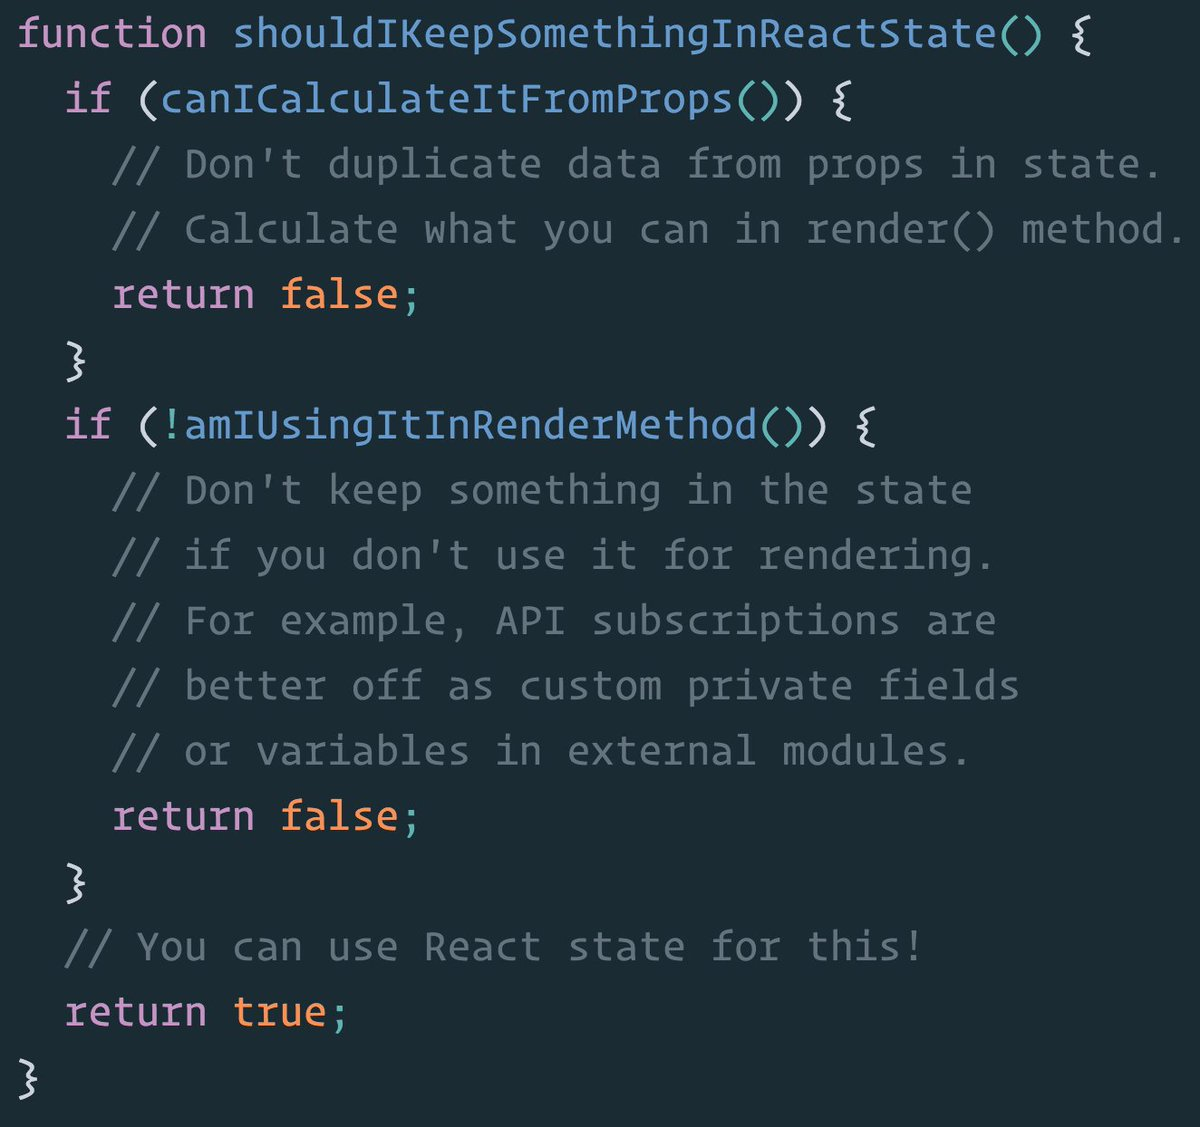
\includegraphics[width=.8\textwidth]{images/dan-cheat-sheet}
\end{figure}


\section{Prop types}

Мы ставим перед собой цель, создавать переиспользуемые компоненты, поэтому нам нужно описывать интерфейс этих компонент удобным для пользователей этих компонент образом.

React из коробки позволяет нам описывать, какие параметры ожидает компонент и простые правила валидации к ним. Привила позволяют указывать, какого типа данных должны быть параметры, а также являются ли параметры обязательными. Помимо этого React позволяет определять пользовательские функции проверки параметров.

Посмотрим на простой пример:

\begin{lstlisting}
const Button = ({ text }) => <button>{text}</button>
Button.propTypes = {
  text: React.PropTypes.string,
}
\end{lstlisting}

В этом примере мы создаем простую компонент-функцию, которая должна получать один параметр $text$, который должен быть типа $string$.

Теперь каждый, кто попытается воспользоваться данным компонентом, сможет легко понять, что ему нужно передавать даже без детального чтения кода.

Но что если компонент вообще не сможет работать, если ему не передать определенный параметр? В этом случае этот параметр можно указать как обязательный:

\begin{lstlisting}
Button.propTypes = {
  text: React.PropTypes.string.isRequired,
}
\end{lstlisting}

В этом случае кто-либо, кто создаст такой компонент, не передав обязательный параметр, получат следующую ошибку:

\begin{quotation}
\textbf{Failed prop type: Required prop `text` was not specified in `Button`.}
\end{quotation}

Важно понимать, что предупреждение об ошибке мы получим только в режиме разработки. В релизной сборке валидация с $propTypes$ выключается в целях улучшения производительности.

React предоставляет возможность проверки множества типов параметров: от чисел до массивов и компонент.

Если мы хотим, чтобы компонент работал с данными разных типов, передаваемых через один параметр, то можем использовать функцию \textbf{oneOf}, которая позволяет указать список разных типов для одного параметра.

Также стоит стараться передавать через параметры только примитивные типы, так как они лучше поддаются отладке и терстированию.

Передача примитивов также позволяет быстрее находить разбухающие интерфейсы у компонент. Если компонент начинает требовать все больше и больше параметров, то возможно он содержит больше логики чем должен и нарушает принцип единственности ответственности.

Если мы замечаем, что компонент получает множество параметров, которые слабо связаны логикой приложение, то можно попробовать разделить этот компонент на два независимых.

Однако нам все равно достаточно часто приходится передавать компонентам объекты. В этом случае для валидации следует использовать функцию $shape$.

Функция $shape$ позволяет определить параметр типа объект, а также определить тип всех полей, которые должны быть у этого объекта, которые в свою очередь тоже могут быть объектами.

Например, если мы создадим компонент $Profile$, который ожидает объект с именем и фамилией пользователя, то мы можем создать следующие $propTypes$:

\begin{lstlisting}
const Profile = ({ user }) =>(
  <div>{user.name} {user.surname}</div>
)
Profile.propTypes = {
  user: React.PropTypes.shape({
    name: React.PropTypes.string.isRequired,
    surname: React.PropTypes.string,
  }).isRequired,
}
\end{lstlisting}

Если же ни одного из стандартных методов валидации React нам не подходят, то мы можем определить собственную функцию проверки:

\begin{lstlisting}
user: React.PropTypes.shape({
  age: (props, propName) => {
    if (!(props[propName] > 0 && props[propName] < 100)) {
      return new Error(`${propName} must be between 1 and 99`)
    }
    return null
  },
})
\end{lstlisting}

Например, в примере выше мы проверяем, что возраст находится в определенном числовом промежутке. Если же возраст выйдет за этот промежуток, то мы увидим соответствующую ошибку в консоли.

\subsection*{React Docgen}

Хорошо описанные $propTypes$ уже значительное облегчение жизни тем, кто будет пользоваться нашими компонентами. Но мы можем пойти дальше и еще больше упростить их использование.

Когда количество компонентов значительно возрастает, то появляется проблема поиска необходимого компонента среди многих, особенно для новых членов проекта.

Но если мы поддерживали $propTypes$ в хорошем состоянии, то мы можем автоматически создавать из них документацию.

Для этого мы можем использовать библиотеку $react-docgen$, которую можно установить следующей командой:

\begin{lstlisting}
npm install --global react-docgen
\end{lstlisting}

React Docgen проходит по файлу с компонентом и достает, необходимую для него информацию, из $propTypes$ и комментариев.

Например, если у нас есть компонент:

\begin{lstlisting}
const Button = ({ text }) => <button>{text}</button>
Button.propTypes = {
  text: React.PropTypes.string,
}
\end{lstlisting}

И мы запустим:

\begin{lstlisting}
react-docgen button.js
\end{lstlisting}

Мы получим следующий результат;

\begin{lstlisting}
{
  "description": "",
  "methods": [],
  "props": {
    "text": {
      "type": {
        "name": "string" 
      },
      "required": false,
      "description": ""
    } 
  }
}
\end{lstlisting}

Этот JSON представляет собой описание интерфейса компонента. Как вы видите, в него попали поля и их типы, описанные в $propTypes$.

Также мы можем добавить комментарий к нашему компоненту:

\begin{lstlisting}
/**
 * A generic button with text.
 */
const Button = ({ text }) => <button>{text}</button>
Button.propTypes = {
  /**
   * The text of the button.
   */
  text: React.PropTypes.string,
}
\end{lstlisting}

Если мы снова запустим Docgen, то получим:

\begin{lstlisting}
{
  "description": "A generic button with text.",
  "methods": [],
  "props": {
    "text": {
      "type": {
        "name": "string"
      },
      "required": false,
      "description": "The text of the button."
    }
  }
}
\end{lstlisting}

Теперь, с этим описанием интерфейса в формате JSON мы можем создать документацию и использовать ее внутри команды.

Результат работы Docgen имеет простой формат, поэтому не составляет никакого труда создать страницу с документацией на его основе.

Один из ярких примеров использования React Docgen - документация библиотеки $Material UI$, где вся документация создана на основе исходного кода библиотеки.


\section{Переиспользуемые компоненты}

Мы уже хорошо разобрались с тем как создавать компоненты, как использовать внутреннее состояние компонент и как сделать их переиспользуемыми с помощью $propTypes$.

Давайте теперь, вооружившись всеми полученными знаниями, попробуем сделать из непереиспользуемыех компонент переиспользуемые.

Предположим, что у нас есть компонент, который загружает список постов через API сервера и отображает их на экране.

Это упрощенный пример, но он хорошо подходит, чтобы показать все этапы создания переиспользуемого компонента.

Создадим класс посредством его наследования от React.Component:

\begin{lstlisting}
class PostList extends React.Component
\end{lstlisting}

Затем создадим конструктор и добавим загрузку данных в $componentDidMount$:

\begin{lstlisting}
constructor(props) {
  super(props)
  this.state = {
    posts: [],
  } 
}
componentDidMount() {
  Posts.fetch().then(posts => {
    this.setState({ posts })
  })
}
\end{lstlisting}

Во $state$ компонента только одно поле $posts$, в котором мы будем хранить посты и которое инициализируется пустым массивом.

В $componentDidMount$ вызывается API сервера, для получения списка постов. По окончанию запроса посты сохраняются в $state$ компонента с помощью метода $setState$.

Это распространенный паттерн загрузки данных, другие варианты детальнее мы рассмотрим в Главе 5.

$Posts$ - это вспомогательный класс, который содержит логику общения с сервером. Сейчас для нас важно только то, что этот класс имеет метод $fetch$, который возвращает $Promise$, который при успешном выполнении вернет список постов.

Теперь мы можем отобразить список постов:

\begin{lstlisting}
render() {
  return (
    <ul>
      {this.state.posts.map(post => (
        <li key={post.id}>
          <h1>{post.title}</h1>
          {post.excerpt && <p>{post.excerpt}</p>}
        </li> ))}
    </ul> 
  )
}
\end{lstlisting}

Внутри метода $render$ мы обходим все посты и для каждого создаем элемент $<li>$.

Мы полагаем, что у поста всегда есть поле $title$ и безусловно показываем его внутри $<h1>$. Поле же $post.excerpt$ мы считаем необязательным и отображаем только при наличии.

Теперь представим другой компонент. Пусть он отображает список пользователей, которые получает из $props$, а не из собственного состояния:

\begin{lstlisting}
const UserList = ({ users }) => (
  <ul>
    {users.map(user => (
      <li key={user.id}>
        <h1>{user.username}</h1>
        {user.bio && <p>{user.bio}</p>}
      </li>
      )
    )} 
  </ul>
)
\end{lstlisting}

Данный компонент отображает список пользователей очень похожим на отображение постов способом.

Отличие в том, что теперь вместо $title$ отображается $username$ и опциональное поле теперь $bio$ пользователя вместо $excerpt$ поста. 

Дублирующийся код как правило считаются плохим звоночком, так что давайте разбираться как React позволяет следовать правилу \textbf{Не повторяйся (Don't Repeat Yourself, DRY)}. Прежде всего мы можем создать отдельный компонент $List$, в который вынесем логику отображения списков, отделив ее от самих данных. Главным требованием является возможность передать ключи полей по которым мы сможем получить данные, чтобы иметь возможность брать нужные данные из разных типов объектов.

Чтобы сделать это, мы определим два параметра: $titleKey$ для передачи ключа, по которому мы получим значение для  обязательного поля, и $textKey$ для передачи ключа опционального поля.

Параметры нашего нового компонента будут выглядеть следующим образом:

\begin{lstlisting}
List.propTypes = {
  collection: React.PropTypes.array,
  textKey: React.PropTypes.string,
  titleKey: React.PropTypes.string,
}
\end{lstlisting}

Так как $List$ не будет обладать своим собственным состоянием, мы можем его создать как компонент-функцию:

\begin{lstlisting}
const List = ({ collection, textKey, titleKey }) => (
  <ul>
    {collection.map(item =>
      <Item
        key={item.id}
        text={item[textKey]}
        title={item[titleKey]}
      /> 
    )}
  </ul> 
)
\end{lstlisting}

Компонент $List$ получает через $props$ коллекцию объектов, проходит по ним и преобразует в элементы $Item$, который мы скоро реализуем. Также в дочерний элемент мы передаем $text$ и $title$, который получаем с помощью полученных ключей из элементов коллекции.

Компонент $Item$ будет максимально простым и чистым:

\begin{lstlisting}
const Item = ({ text, title }) => (
  <li>
    <h1>{title}</h1>
    {text && <p>{text}</p>}
  </li>
)

Item.propTypes = {
  text: React.PropTypes.string,
  title: React.PropTypes.string,
}
\end{lstlisting}

Таким образом мы создали два компонента с достаточно простыми интерфейсами, чтобы с их помощью отображать пользователей, посты или что-либо еще. При этом такие небольшие компоненты очень удобны в поддержке и тестировании.

Отлично, теперь мы можем переписать наши исходные компоненты с использованием новых вспомогательных компонент.

Метод $render$ компонента $PostsList$ будет выглядеть следующим образом:

\begin{lstlisting}
render() {
  return (
    <List
      collection={this.state.posts}
      textKey="excerpt"
      titleKey="title"
    />
  )
}
\end{lstlisting}

А компонент-функция $UserList$ следующим:

\begin{lstlisting}
const UserList = ({ users }) => (
  <List
    collection={users}
    textKey="bio"
    titleKey="username"
  /> 
)
\end{lstlisting}

Таким образом мы из узкоспециализированных компонент получили базовые компоненты, которые могут быть переиспользованы в будущем.

Мы также можем использовать $react-docgen$ для генерации документации для полученных нами компонент.

Также теперь в случае необходимости расширения данного отображения, которое пока состоит из двух текстовых полей, нам будет достаточно поменять его в одном компоненте $Item$, а не в множестве узкоспециализированных компонент.

Например, если нам понадобится в случае слишком длинной строки урезать ее и показывать троеточие, нам будет достаточно добавить эту логику внутрь одного компонента.

\section{Living style guides}

Использование переиспользуемых компонент с простыми интерфейсами - хороший способ сократить количество дублирующегося кода в проекте, но это не единственная причина, чтобы сосредоточиться на переиспользуемости.

Если вы создаете простые и понятные компоненты с чистыми интерфейсами, которые хорошо отделены абстракциями от конкретных данных, то эти компоненты можно объединить в библиотеку компонент и использовать за пределами команды. Такая библиотека будет представлять из себя набор готовых к использованию блоков, которыми можно будет поделиться с другими командами, дизайнерами или выложить ее в open source.

Очень часто новым членам команды может быть сложно понять, какие компоненты уже есть, а какие нужно реализовать. Решением этой проблемы может быть создание Style guide'а, которое бы позволило распространять не только сами компоненты, но и примеры их использования.

По сути style guide - это собранное визуальное представление всех единичных компонентов, которые уже реализованы в проекте. Это очень удобный способ сохранять единый стиль всех компонент среди множества разработчиков разного уровня. 

К сожалению, создание style guide'а не всегда является простой задачей, так как из-за меняющихся требований может появиться множество дублирующихся компонент с небольшими отличиями, решающие какие-то локальные проблемы. Тем не менее React позволяет без значительных усилий создавать такой род документации, что может окупить немало времени в будущем.

Но не только React может вам помочь создать библиотеку визуальных компонентов из кода самих компонент. Есть инструменты, которые помогают решить эту проблему, один из которых $react-storybook$.

React Storybook изолирует компоненты, предоставляя вам возможность создавать компоненты без запуска всего приложения, что помогает в тестировании и разработке.

Как видно из названия библиотеки React Storybook позволяет создавать истории для отображения разных состояний компонента. Например, если вы пишите TO-DO приложение, то вы можете создать две истории для отображения выбранного и невыбранного состояний элемента.

Давайте попробуем применить эту библиотеку к примеру с компонентом $List$. Прежде всего нам нужно установить Storybook:

%npm install --save @kadira/react-storybook-addon

Теперь мы можем начать создавать истории.

В нашем примере компонент $Item$ требует обязательный параметр $title$ и опциональный $text$, в этом случае мы можем создать как минимум две истории.

Обычно истории хранят в директории $stories$ внутри проекта, но в целом никто не запрещает использовать любую удобную для вас директорию.

Внутри этой директории можно создать специально файл для каждой из компонент.

В нашем случае создадим файл $list.js$. В этом файле обязательно необходимо добавить импорт основной функции библиотеки:

\begin{lstlisting}
import { storiesOf } from '@kadira/storybook'
\end{lstlisting}

Дальше мы можем создать истории следующим образом:

\begin{lstlisting}
storiesOf('List', module)
  .add('without text field', () => (
    <List collection={posts} titleKey="title" />
  ))
\end{lstlisting}

Функция $storiesOf$ принимает аргументом название компонента и позволяет добавить для него множество историй. Каждая история включает в себя описание и функцию, которая создает необходимый компонент.

В нашем случае $posts$ может быть объектом вида:

\begin{lstlisting}
const posts = [
  {
    id: 1,
    title: 'Create Apps with No Configuration',
  },
  {
    id: 2,
    title: 'Mixins Considered Harmful',
  },
]
\end{lstlisting}

Перед запуском Storybook и создания нашей визуальной коллекции нам необходимо настроить библиотеку. Для этого необходимо создать директорию $.storybook$. 

Внутри этой директории нам нужно создать файл $config.js$ для загрузки наших историй:

\begin{lstlisting}
import { configure } from '@kadira/storybook'
function loadStories() {
  require('../src/stories/list')
}
configure(loadStories, module)
\end{lstlisting}

Сначала мы загружаем функцию $configure$ из библиотеки, а затем описываем функцию для загрузки историй по путям к их файлам.

И последний шаг, если мы хотим, чтобы storybook с нашими компонентами был доступен из браузера, мы можем добавить специальный скрипт в package.json:

\begin{lstlisting}
"storybook": "start-storybook -p 9001"
\end{lstlisting}

Теперь мы можем запустить storybook:

\begin{lstlisting}
npm run storybook
\end{lstlisting}

И открыть в браузере $http://localhost:9001$.

Теперь мы можем увидеть интерфейс storybook. Слева находится список наших историй. Если мы нажмем на историю, то справа увидим соответствующий ей компонент.

Отлично, теперь у нас есть визуальная документация наших компонент, чтобы все члены команды, в том числе продуктовые менеджеры и дизайнеры, имели представление о существующей базе готовых компонентов.

В завершение мы можем создать еще одну историю.

Наш лист умеет отображать элементы с $title$ и $text$, поэтому добавим второй атрибут в список постов:

\begin{lstlisting}
const posts = [
  {
    id: 1,
    title: 'Create Apps with No Configuration',
    excerpt: 'Create React App is a new officially supported...',
  }, 
  {
    id: 2,
    title: 'Mixins Considered Harmful',
    excerpt: '"How do I share the code between several...',
  }
]
\end{lstlisting}

После этого добавим еще одну историю, где передадим оба параметра:

\begin{lstlisting}
.add('with text field', () => (
  <List collection={posts} titleKey="title" textKey="excerpt" />
))
\end{lstlisting}

Если мы сейчас вернемся в браузер, то увидим, что наша страница автоматически обновилась, и добавилась вторая история.

Таким образом для сложных компонентов мы можем добавить любое количество историй, чтобы показать все состояния, в которых они могут находиться.

\section{Заключение}

Поздравляю, мы разобрались с созданием переиспользуемых компонент.

В этой главе мы детально посмотрели как можно создавать компоненты и в чем различие между компонент-функциями и компонентами с внутренним состоянием. Также мы изучили как осуществляется изменение состояния React компонент и как это приводит к перерисовке компонента. Помимо этого мы посмотрели как описывать параметры компонента и как это помогает в совместной работе надо общими элементами.

И в конце мы посмотрели на примеры превращения узкоспециализированных компонент в переиспользуемые посредством вынесения общей логики в достаточно абстрактные базовые компоненты.

Теперь пришло время посмотреть на разные техники комбинации компонентов между собой.




\end{document}










